\documentclass[a4paper,12pt]{article}

\usepackage[utf8]{inputenc}
\usepackage[russian]{babel}
\usepackage{graphicx}
\usepackage{geometry}
\usepackage{hyperref}
\usepackage{listings} % Для вставки и подсветки кода
\usepackage{xcolor}   % Для использования цветов
\usepackage[T2A]{fontenc} % Для поддержки кириллицы
\usepackage[utf8]{inputenc} % Для поддержки UTF-8
\lstset{
    language=SQL,               % Язык программирования (SQL)
    basicstyle=\ttfamily\small, % Стиль текста
    keywordstyle=\color{blue},  % Стиль ключевых слов (синий)
    commentstyle=\color{green}, % Стиль комментариев (зелёный)
    stringstyle=\color{red},    % Стиль строк (красный)
    numbers=left,               % Нумерация строк слева
    numberstyle=\tiny,          % Стиль номеров строк
    stepnumber=1,               % Шаг нумерации строк
    numbersep=5pt,              % Отступ номеров строк от кода
    backgroundcolor=\color{white}, % Цвет фона
    showspaces=false,           % Показывать пробелы
    showstringspaces=false,     % Показывать пробелы в строках
    showtabs=false,             % Показывать табуляцию
    frame=single,               % Рамка вокруг кода
    rulecolor=\color{black},    % Цвет рамки
    tabsize=2,                  % Размер табуляции
    captionpos=b,               % Позиция заголовка (bottom)
    breaklines=true,            % Переносить длинные строки
    breakatwhitespace=true,     % Переносить только по пробелам
    escapeinside={\%*}{*)},     % Возможность вставки LaTeX-кода внутри листинга
    morekeywords={CREATE, TABLE, SELECT, INSERT, UPDATE, DELETE, WHERE, FROM, INTO, VALUES, SET, VARCHAR, INT, PRIMARY, KEY, NOT, NULL, AUTO_INCREMENT}, % Дополнительные ключевые слова
    literate=                    % Поддержка кириллицы
        {а}{{\selectfont\char224}}1
        {б}{{\selectfont\char225}}1
        {в}{{\selectfont\char226}}1
        {г}{{\selectfont\char227}}1
        {д}{{\selectfont\char228}}1
        {е}{{\selectfont\char229}}1
        {ё}{{\selectfont\char184}}1
        {ж}{{\selectfont\char230}}1
        {з}{{\selectfont\char231}}1
        {и}{{\selectfont\char232}}1
        {й}{{\selectfont\char233}}1
        {к}{{\selectfont\char234}}1
        {л}{{\selectfont\char235}}1
        {м}{{\selectfont\char236}}1
        {н}{{\selectfont\char237}}1
        {о}{{\selectfont\char238}}1
        {п}{{\selectfont\char239}}1
        {р}{{\selectfont\char240}}1
        {с}{{\selectfont\char241}}1
        {т}{{\selectfont\char242}}1
        {у}{{\selectfont\char243}}1
        {ф}{{\selectfont\char244}}1
        {х}{{\selectfont\char245}}1
        {ц}{{\selectfont\char246}}1
        {ч}{{\selectfont\char247}}1
        {ш}{{\selectfont\char248}}1
        {щ}{{\selectfont\char249}}1
        {ъ}{{\selectfont\char250}}1
        {ы}{{\selectfont\char251}}1
        {ь}{{\selectfont\char252}}1
        {э}{{\selectfont\char253}}1
        {ю}{{\selectfont\char254}}1
        {я}{{\selectfont\char255}}1
        {А}{{\selectfont\char192}}1
        {Б}{{\selectfont\char193}}1
        {В}{{\selectfont\char194}}1
        {Г}{{\selectfont\char195}}1
        {Д}{{\selectfont\char196}}1
        {Е}{{\selectfont\char197}}1
        {Ё}{{\selectfont\char168}}1
        {Ж}{{\selectfont\char198}}1
        {З}{{\selectfont\char199}}1
        {И}{{\selectfont\char200}}1
        {Й}{{\selectfont\char201}}1
        {К}{{\selectfont\char202}}1
        {Л}{{\selectfont\char203}}1
        {М}{{\selectfont\char204}}1
        {Н}{{\selectfont\char205}}1
        {О}{{\selectfont\char206}}1
        {П}{{\selectfont\char207}}1
        {Р}{{\selectfont\char208}}1
        {С}{{\selectfont\char209}}1
        {Т}{{\selectfont\char210}}1
        {У}{{\selectfont\char211}}1
        {Ф}{{\selectfont\char212}}1
        {Х}{{\selectfont\char213}}1
        {Ц}{{\selectfont\char214}}1
        {Ч}{{\selectfont\char215}}1
        {Ш}{{\selectfont\char216}}1
        {Щ}{{\selectfont\char217}}1
        {Ъ}{{\selectfont\char218}}1
        {Ы}{{\selectfont\char219}}1
        {Ь}{{\selectfont\char220}}1
        {Э}{{\selectfont\char221}}1
        {Ю}{{\selectfont\char222}}1
        {Я}{{\selectfont\char223}}1
}
\geometry{a4paper, margin=1in}

\begin{document}
a
\newpage

\section{Задание}

\subsection{Туристическое агентство}

Клиент обращается в агентство, где совместно с консультантом подбирается туристическая поездка, согласовываются отель, транспорт, культурная программа. Агентство обеспечивает бронирование мест в гостинице, а также по желанию клиента может, как участвовать, так и нет в организации авиаперелёта, трансфере от/до аэропорта, оформлении виз. В процессе подготовки поездки могут возникать ситуации, требующие дополнительного согласования с клиентом: изменение стоимости, сроков, отеля и так далее. Не всегда подобные вопросы удается решать, и поездка в таком случае отменяется.

\section{Описание предметной области}

Система предназначена для удобного хранения, отображения и редактирования информации о туристических поездках клиентов. Участниками системы являются менеджеры и клиенты. Все участники могут выполнять базовые операции в системе, такие как вход, регистрация, просмотр информации о поездках.

В результате работы были разработаны следующие модели:

\begin{enumerate}
    \item Концептуальная модель предметной области

          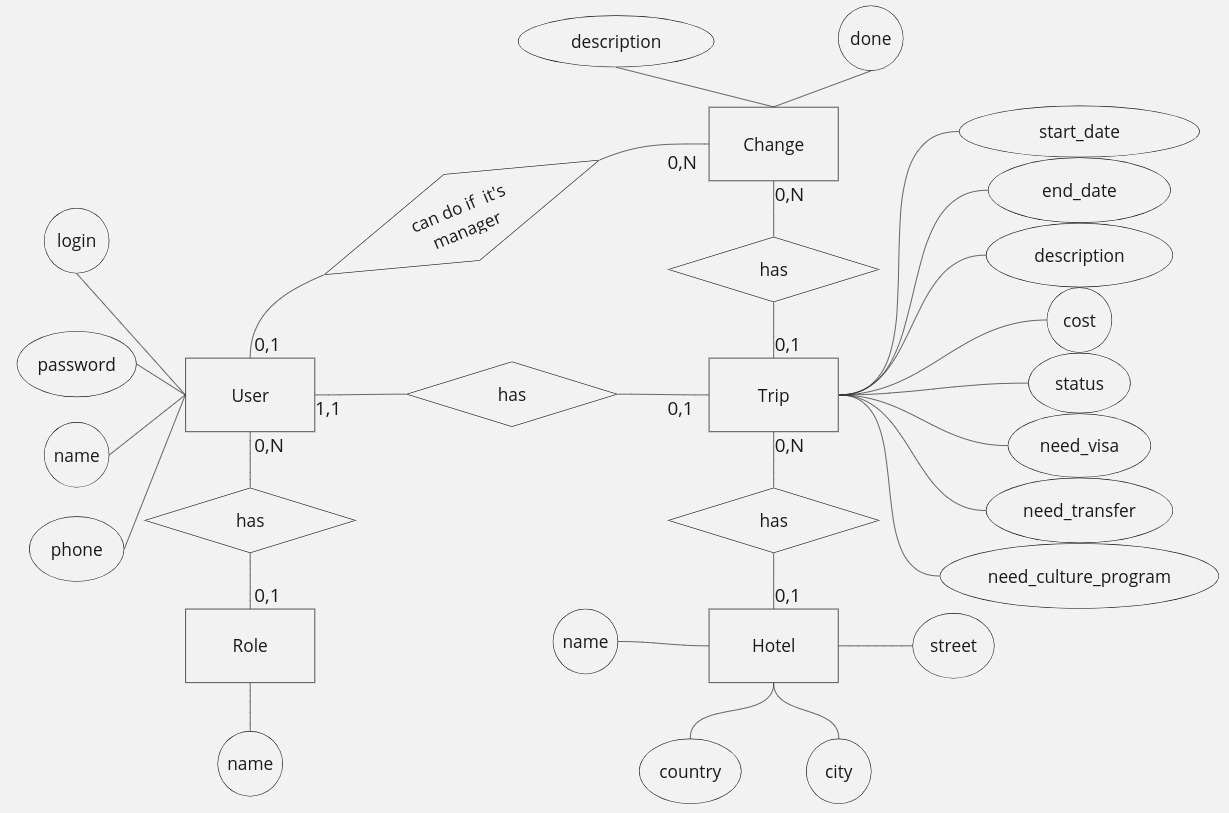
\includegraphics[width=\textwidth]{media/ER.jpg}

          Описание концептуальной модели такое же, как у базы данных (пункт 3.2)

    \item Функциональная модель

          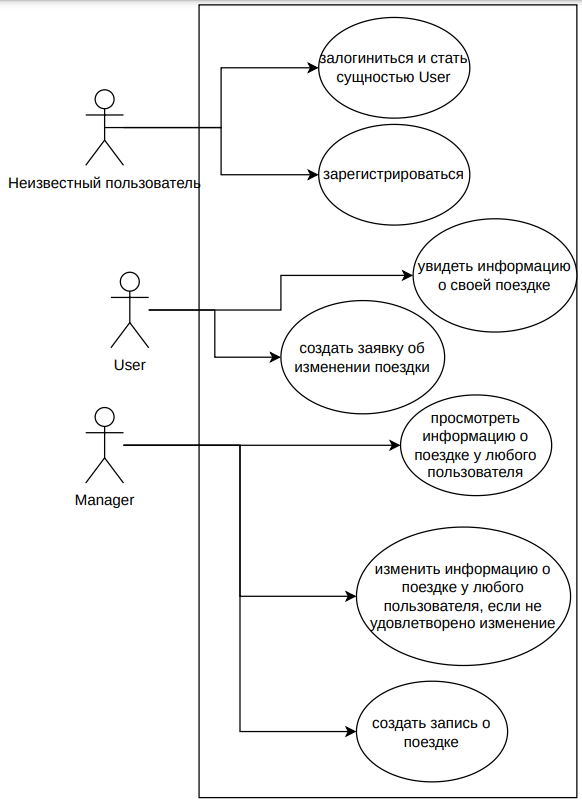
\includegraphics[width=4.856262029746282in, height=6.687497812773404in]{media/f_model.png}

          Неизвестный пользователь может залогиниться и стать пользователем или зарегистрироваться.

          Пользователь может просматривать информацию о своей поездке и отправить заявку об изменении своей поездки.

          Менеджер может посмотреть информацию о поездке у любого пользователя, изменить информацию о поездке у любого пользователя, если не сделано изменение, посланное клиентом, создать запись о поездке для клиента.

    \item Алгоритмическая модель

          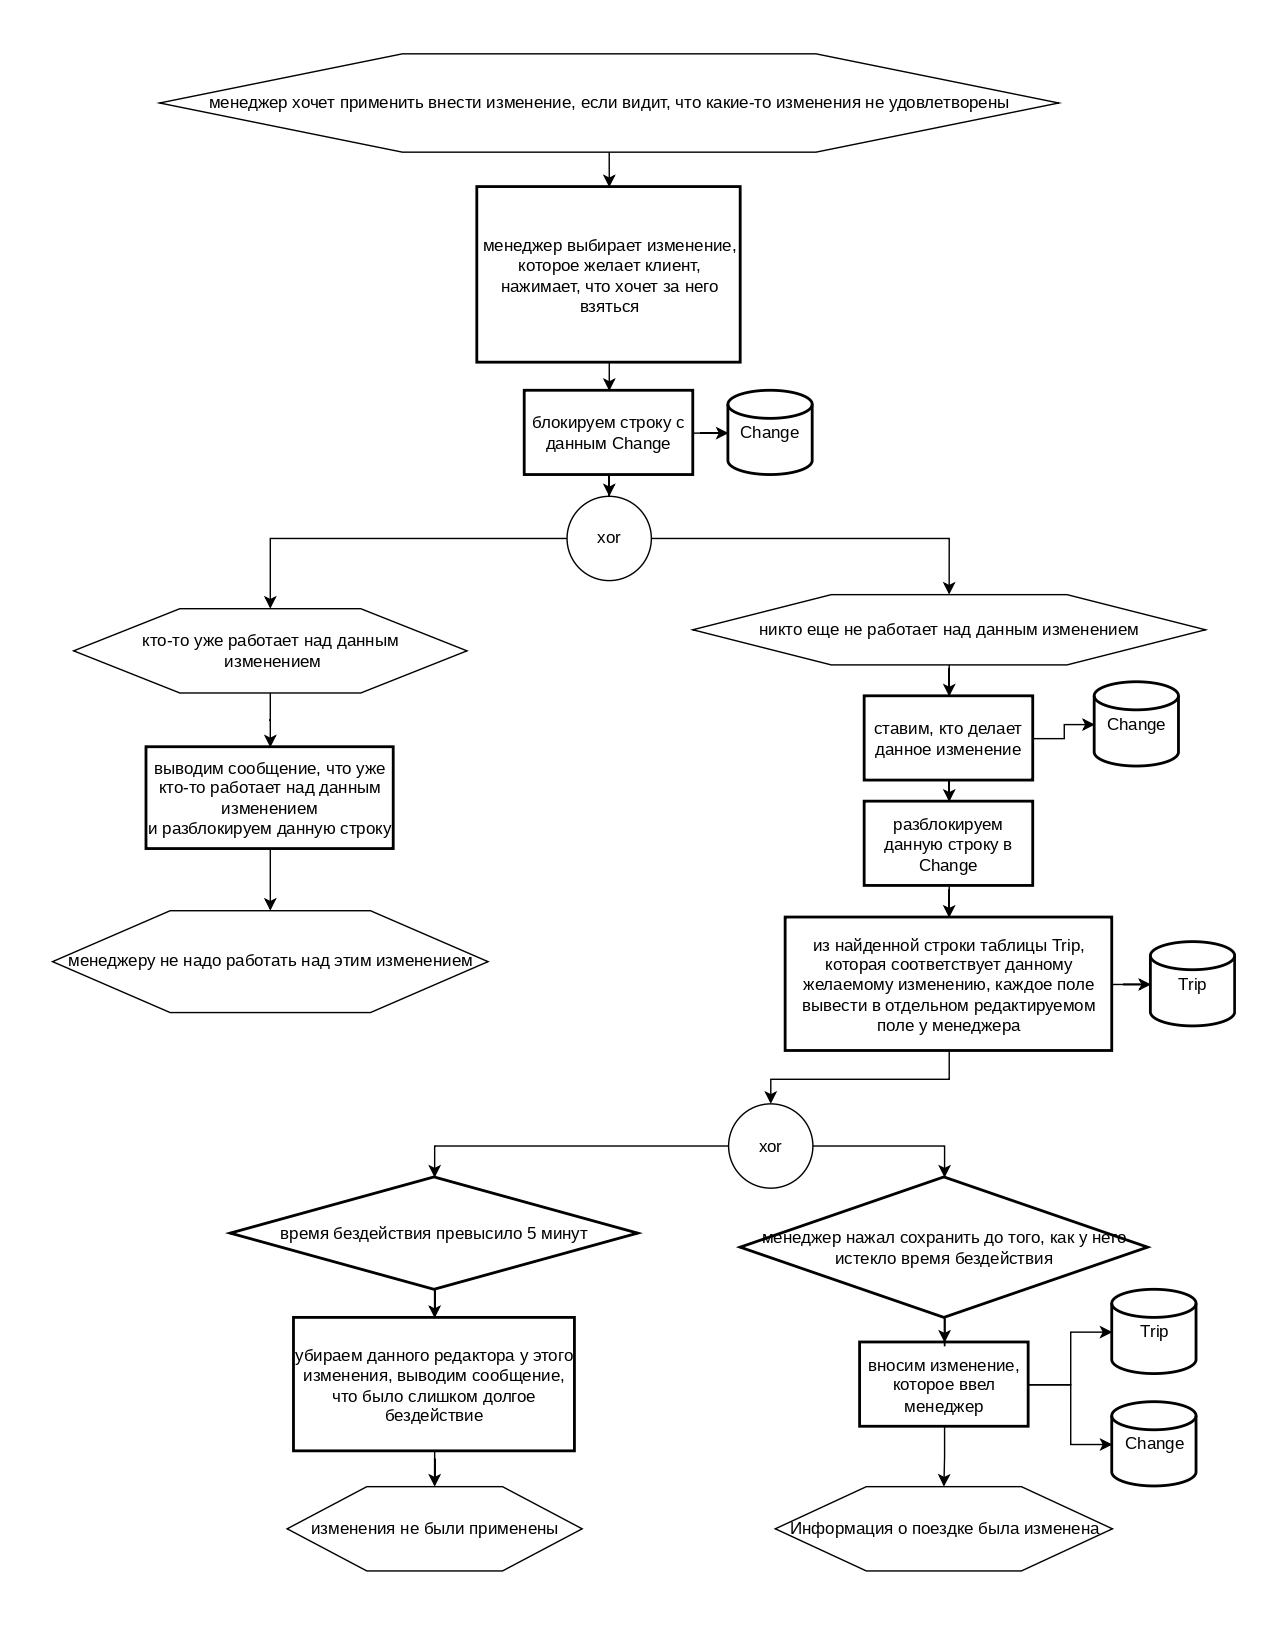
\includegraphics[width=\textwidth]{media/alg_model.jpg}

          Здесь представлен алгоритм для редактирования информации о поездке менеджером. Ключевым моментом является то, что блокируется данная заявка на изменение в базе данных, проверяется, что данная заявка никем не обрабатывается, после чего в данную заявку на изменение помещается id менеджера, чтобы никакой другой менеджер уже не смог работать над данной заявкой. Только при успешном прохождении данных этапов менеджер сможет работать над данной заявкой на изменение.

    \item Модель базы данных

          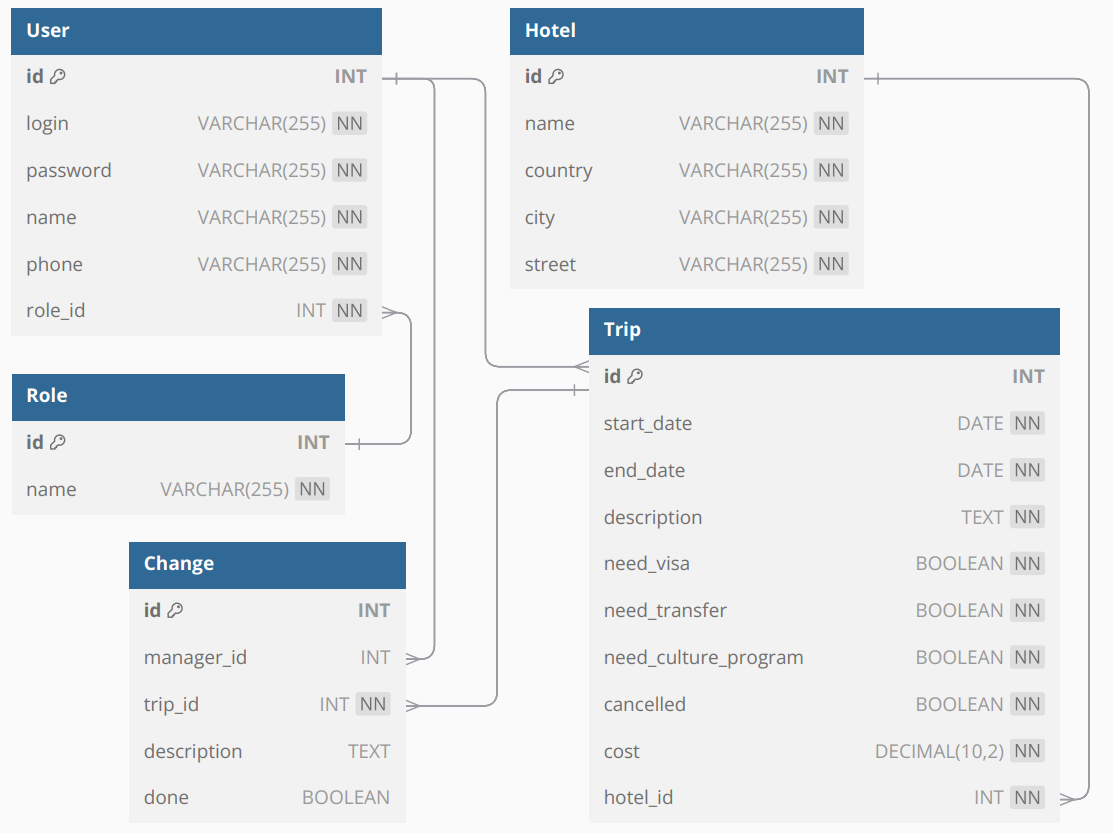
\includegraphics[width=6.010415573053368in, height=4.5in]{media/base_model.png}

          Описание модели базы данных такое же, как у базы данных (пункт 3.2)
\end{enumerate}

\section{Описание реализации}

\subsection{Описание программных файлов}

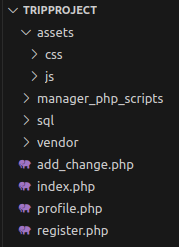
\includegraphics[width=2.317518591426072in, height=3.1979166666666665in]{media/files_description.png}

В процессе разработки код был разбит на файлы и директории.

\begin{itemize}
    \item \texttt{assets} содержит в себе стили для страниц и javascript код для валидации авторизации и регистрации.
    \item \texttt{vendor} содержит в себе файлы для подключения к базе данных, регистрации, авторизации, выхода из аккаунта.
    \item В папке \texttt{sql} файлы \texttt{create\_db.sql} и \texttt{create\_data.sql} отвечают за создание и заполнение базы данных.
    \item \texttt{index.php} отвечает за стартовую страницу, на которой доступны регистрация и авторизация.
    \item \texttt{register.php} хранит в себе форму для регистрации.
    \item \texttt{profile.php} отвечает за личный кабинет пользователей.
    \item \texttt{add\_change.php} отвечает за добавление заявки на изменение.
    \item В папке \texttt{manager\_php\_scripts} лежат следующие файлы:
          \begin{itemize}
              \item \texttt{create\_trip.php} отвечает за создание поездки менеджером для пользователя.
              \item \texttt{edit\_client.php} отвечает за редактирование поездки менеджером.
              \item \texttt{process\_form.php} отвечает за обработку формы на редактирование поездки.
              \item \texttt{time\_out\_handler.php} отвечает за отмену редактирования поездки менеджером при слишком долгом бездействии.
              \item \texttt{watch\_trip\_info.php} отвечает за простой просмотр информации о поездках клиентов.
          \end{itemize}
\end{itemize}

\subsection{Описание базы данных}

Была использована СУБД MySQL.

\subsubsection{Код для создания таблиц в базе данных:}

\begin{lstlisting}[label={lst:sql-example}]
    CREATE TABLE IF NOT EXISTS `Role` (
        id INT PRIMARY KEY AUTO_INCREMENT,
        name VARCHAR(255) NOT NULL UNIQUE
    );
    INSERT INTO `Role` (id, name) VALUES
    (1, 'user'),
    (2, 'manager');
    
    CREATE TABLE IF NOT EXISTS `Hotel` (
        id INT PRIMARY KEY AUTO_INCREMENT,
        `name` VARCHAR(255) NOT NULL,
        country VARCHAR(255) NOT NULL,
        city VARCHAR(255) NOT NULL,
        street VARCHAR(255) NOT NULL
    );
    
    CREATE TABLE IF NOT EXISTS `User` (
        id INT PRIMARY KEY AUTO_INCREMENT,
        `login` VARCHAR(255) NOT NULL UNIQUE,
        `password` VARCHAR(255) NOT NULL,
        `name` VARCHAR(255) NOT NULL,
        phone VARCHAR(255) NOT NULL,
        role_id INT NOT NULL DEFAULT 1,
        FOREIGN KEY (role_id) REFERENCES `Role`(id)
    );
    
    CREATE TABLE IF NOT EXISTS `Trip` (
        id INT PRIMARY KEY,
        `start_date` DATE NOT NULL DEFAULT CURRENT_DATE,
        end_date DATE NOT NULL DEFAULT CURRENT_DATE,
        `description` TEXT NOT NULL DEFAULT 'Description',
        need_visa BOOLEAN NOT NULL DEFAULT FALSE,
        need_transfer BOOLEAN NOT NULL DEFAULT FALSE,
        need_culture_program BOOLEAN NOT NULL DEFAULT FALSE,
        cancelled BOOLEAN NOT NULL DEFAULT FALSE,
        cost DECIMAL(10, 2) NOT NULL DEFAULT 0,
        hotel_id INT NOT NULL DEFAULT 1,
        FOREIGN KEY (id) REFERENCES `User`(id),
        FOREIGN KEY (hotel_id) REFERENCES `Hotel`(id)
    );
    
    CREATE TABLE IF NOT EXISTS `Change` (
        id INT PRIMARY KEY AUTO_INCREMENT,
        trip_id INT NOT NULL,
        manager_id INT DEFAULT NULL,
        `description` TEXT DEFAULT "Description",
        done BOOLEAN DEFAULT FALSE,
        FOREIGN KEY (manager_id) REFERENCES `User`(id),
        FOREIGN KEY (trip_id) REFERENCES `Trip`(id)
    );
    
    DELIMITER $$
    CREATE TRIGGER after_trip_insert
    AFTER INSERT ON `Trip`
    FOR EACH ROW
    BEGIN
        INSERT INTO `Change` (trip_id, description)
        VALUES (NEW.id, 'automatically generated change');
    END$$
    DELIMITER ;
    
\end{lstlisting}

\begin{itemize}
    \item \texttt{User} (Пользователь) представляет пользователей системы: клиентов и менеджеров.
          \begin{itemize}
              \item \texttt{login} (логин пользователя)
              \item \texttt{password} (пароль пользователя для входа в систему)
              \item \texttt{name} (имя пользователя)
              \item \texttt{phone} (телефон пользователя)
              \item \texttt{role\_id} (id роли, которую он имеет в системе: пользователь либо клиент, либо менеджер)
          \end{itemize}


    \item \texttt{Role} (Роль) описывает роль, которую может иметь пользователь.
          \begin{itemize}
              \item \texttt{name} (имя роли)
          \end{itemize}



    \item \texttt{Trip} (Поездка) описывает поездку, которую клиент может иметь.
          \begin{itemize}
              \item \texttt{start\_date} (дата начала поездки)
              \item \texttt{end\_date} (дата окончания поездки)
              \item \texttt{description} (описание поездки для уточнения важных деталей)
              \item \texttt{need\_visa} (нужна ли пользователю виза)
              \item \texttt{need\_transfer} (нужен ли пользователю трансфер)
              \item \texttt{need\_culture\_program} (нужна ли пользователю культурная программа)
              \item \texttt{cost} (стоимость поездки)
              \item \texttt{hotel\_id} (id отеля, проживание в котором будет включено в стоимость поездки)
              \item \texttt{cancelled} (отменена ли поездка)
          \end{itemize}



    \item \texttt{Hotel} (Отель) описывает отель, который должен входить в поездку.
          \begin{itemize}
              \item \texttt{name} (название отеля)
              \item \texttt{country} (страна, в которой находится отель)
              \item \texttt{city} (город, в котором находится отель)
              \item \texttt{street} (улица, на которой находится отель)
          \end{itemize}



    \item \texttt{Change} (Изменение) описывает изменение, которое хочет внести клиент в поездку.
          \begin{itemize}
              \item \texttt{description} (описание желаемого изменения)
              \item \texttt{trip\_id} (id поездки, к которой относится изменение)
              \item \texttt{meneger\_id} (id менеджера, редактирующего поездку на данный момент)
              \item \texttt{done} (совершено ли изменение)
          \end{itemize}



    \item Триггер для создания поездки. Очевидно, что сразу после создания поездки, ее нужно редактировать.


\end{itemize}

\subsubsection{Код для создания первоначальных данных:}

\begin{lstlisting}[label={lst:sql-example}]
    INSERT INTO `Hotel` (name, country, city, street) VALUES
    ('Отель Солнечный', 'Россия', 'Сочи', 'Курортная 15'),
    ('Отель Звездный', 'Россия', 'Санкт-Петербург', 'Невский проспект 22'),
    ('Отель Горный', 'Россия', 'Красная Поляна', 'Горная 7'),
    ('Отель Морской', 'Россия', 'Калининград', 'Морская 33'),
    ('Отель Лесной', 'Россия', 'Казань', 'Лесная 12');
    
    INSERT INTO `User` (login, password, name, phone, role_id) VALUES
    ('user1', MD5('password1'), 'Иван Иванов', '79100000001', 1),
    ('user2', MD5('password2'), 'Петр Петров', '79100000002', 1),
    ('user3', MD5('password3'), 'Сергей Сергеев', '79100000003', 1),
    ('user4', MD5('password4'), 'Алексей Алексеев', '79100000004', 1),
    ('user5', MD5('password5'), 'Дмитрий Дмитриев', '79100000005', 1),
    ('user6', MD5('password6'), 'Андрей Андреев', '79100000006', 1),
    ('user7', MD5('password7'), 'Николай Николаев', '79100000007', 1),
    ('user8', MD5('password8'), 'Александр Александров', '79100000008', 1),
    ('user9', MD5('password9'), 'Виктор Викторов', '79100000009', 1),
    ('user10', MD5('password10'), 'Евгений Евгеньев', '79100000010', 1);
    
    INSERT INTO `User` (login, password, name, phone, role_id) VALUES
    ('first_manager', MD5('a'), 'Михаил Колесников', '79100000011', 2),
    ('second_manager', MD5('b'), 'Евгений Кондаков', '79100000012', 2);
    
    INSERT INTO `Trip` 
    (id, start_date, end_date, description, need_visa, need_transfer, need_culture_program, cancelled, cost, hotel_id) 
    VALUES
    (1, '2023-10-01', '2023-10-10', 'Поездка в Сочи', FALSE, TRUE, TRUE, FALSE, 50000.00, 2),
    (2, '2023-11-05', '2023-11-15', 'Поездка в Санкт-Петербург', FALSE, FALSE, TRUE, FALSE, 45000.00, 3),
    (3, '2023-12-01', '2023-12-10', 'Поездка в Красную Поляну', FALSE, TRUE, FALSE, FALSE, 60000.00, 4),
    (4, '2024-01-10', '2024-01-20', 'Поездка в Калининград', TRUE, TRUE, TRUE, FALSE, 55000.00, 5),
    (5, '2024-02-15', '2024-02-25', 'Поездка в Казань', FALSE, FALSE, FALSE, FALSE, 40000.00, 6),
    (6, '2024-03-01', '2024-03-10', 'Поездка в Сочи', FALSE, TRUE, TRUE, FALSE, 50000.00, 2),
    (7, '2024-04-05', '2024-04-15', 'Поездка в Санкт-Петербург', FALSE, FALSE, TRUE, FALSE, 45000.00, 3);        
\end{lstlisting}

\subsection{Описание всего разработанного интерфейса со скриншотами}

\begin{itemize}
    \item Страница авторизации

          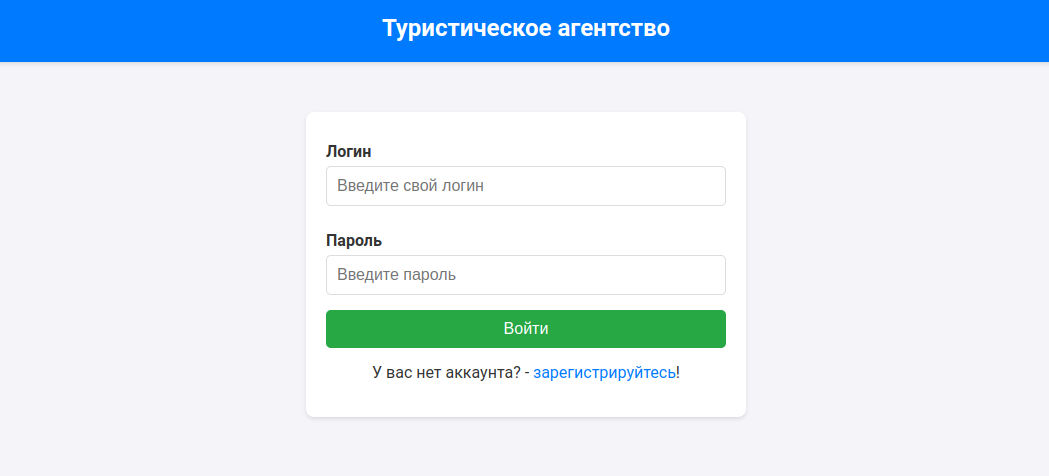
\includegraphics[width=6.260415573053368in, height=2.84375in]{media/login.png}

    \item Страница регистрации

          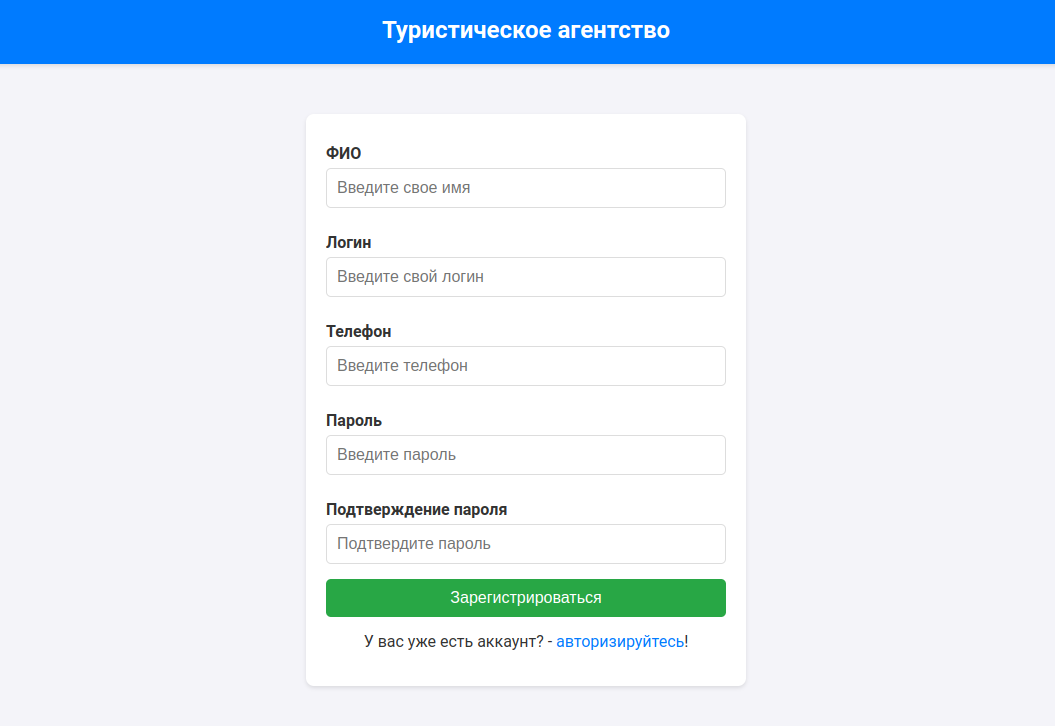
\includegraphics[width=6.260415573053368in, height=4.3125in]{media/reg.png}

    \item Личный кабинет клиента (два варианта, с поездкой и без)

          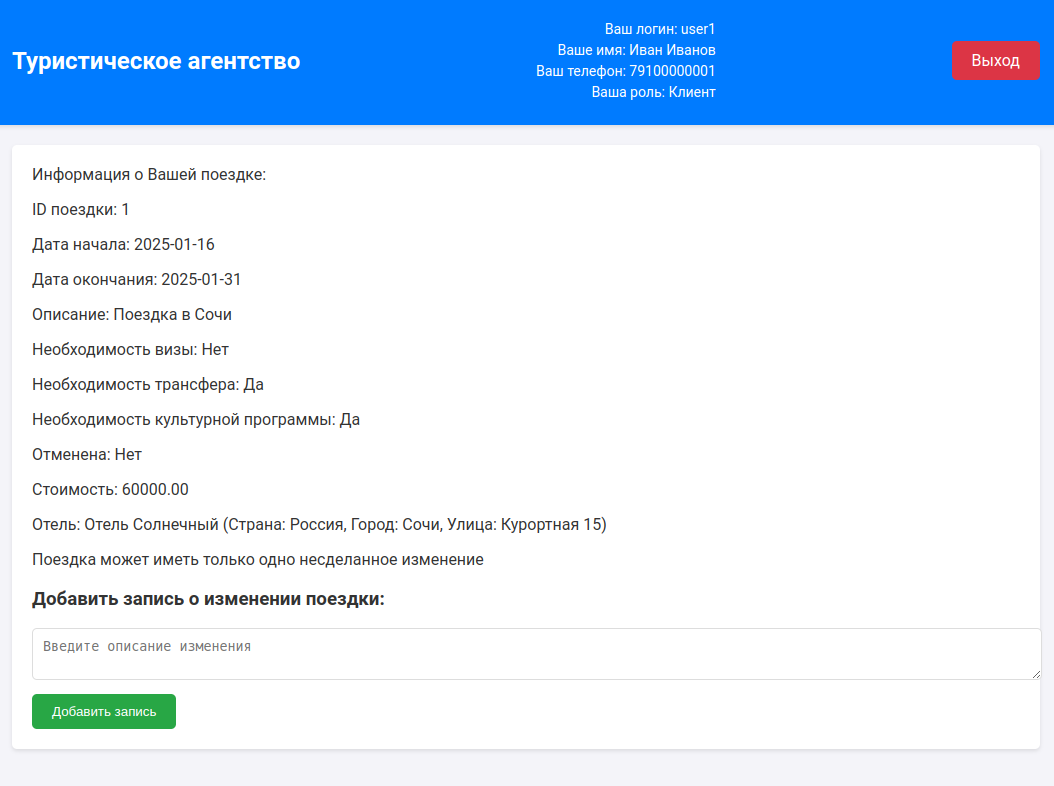
\includegraphics[width=6.260415573053368in, height=4.666666666666667in]{media/client_with.png}

          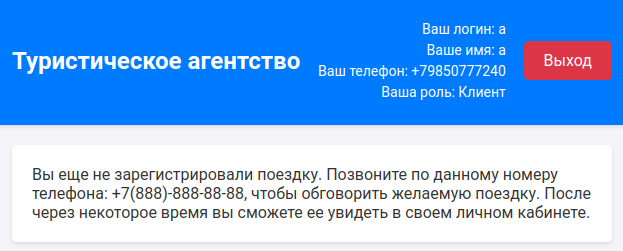
\includegraphics[width=6.260415573053368in, height=2.5208333333333335in]{media/client_without.png}

    \item Личный кабинет менеджера (разбит на два скриншота)

          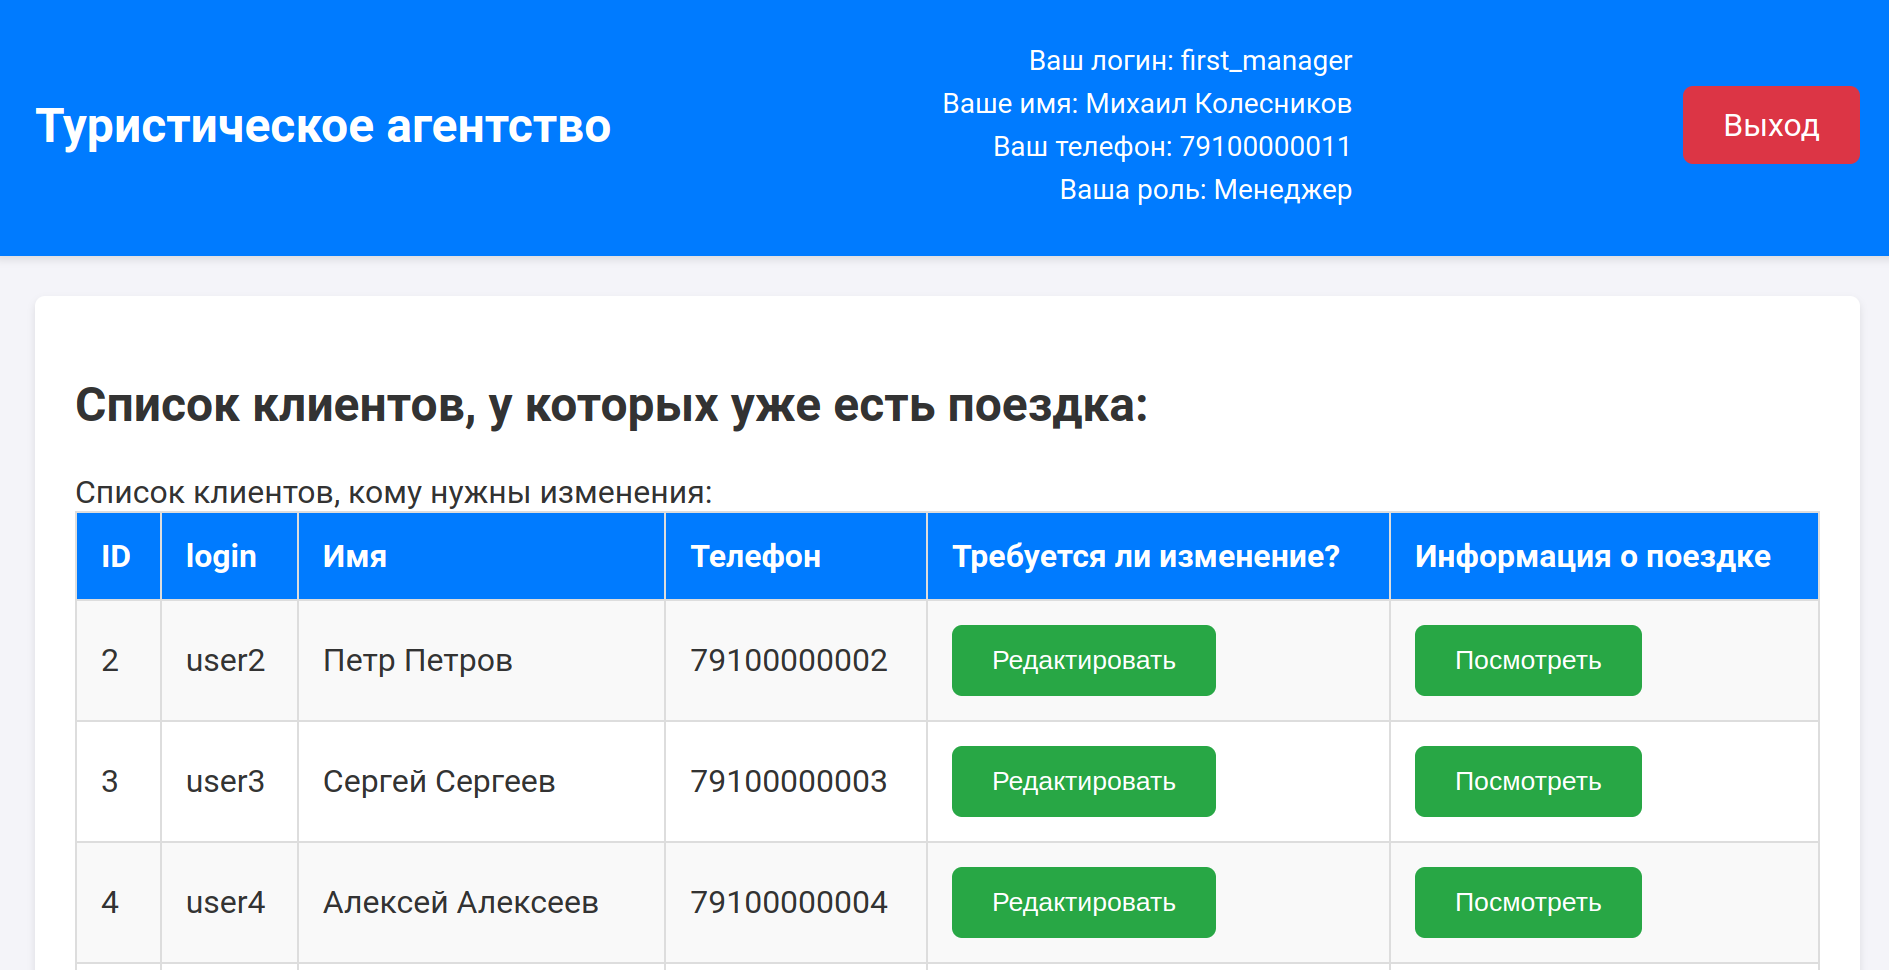
\includegraphics[width=6.260415573053368in, height=3.21875in]{media/manager1.png}

          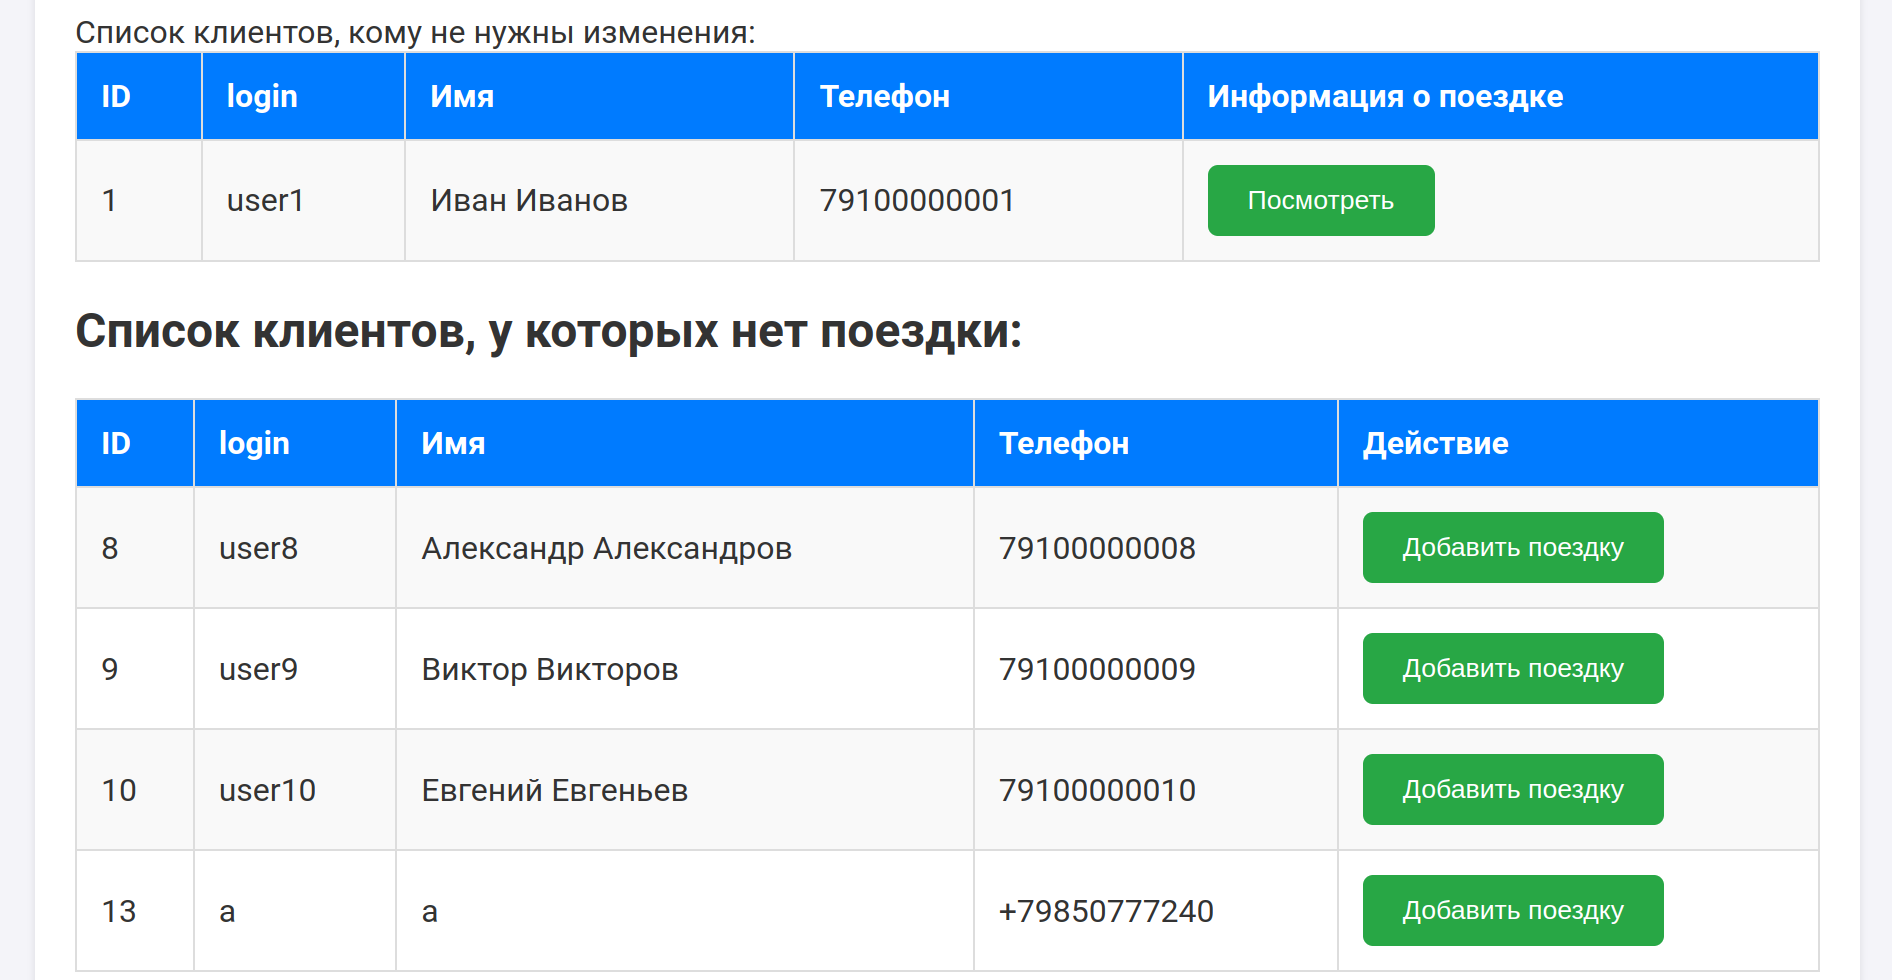
\includegraphics[width=6.260415573053368in, height=3.2395833333333335in]{media/manager2.png}

    \item Страница редактирования поездки менеджером

          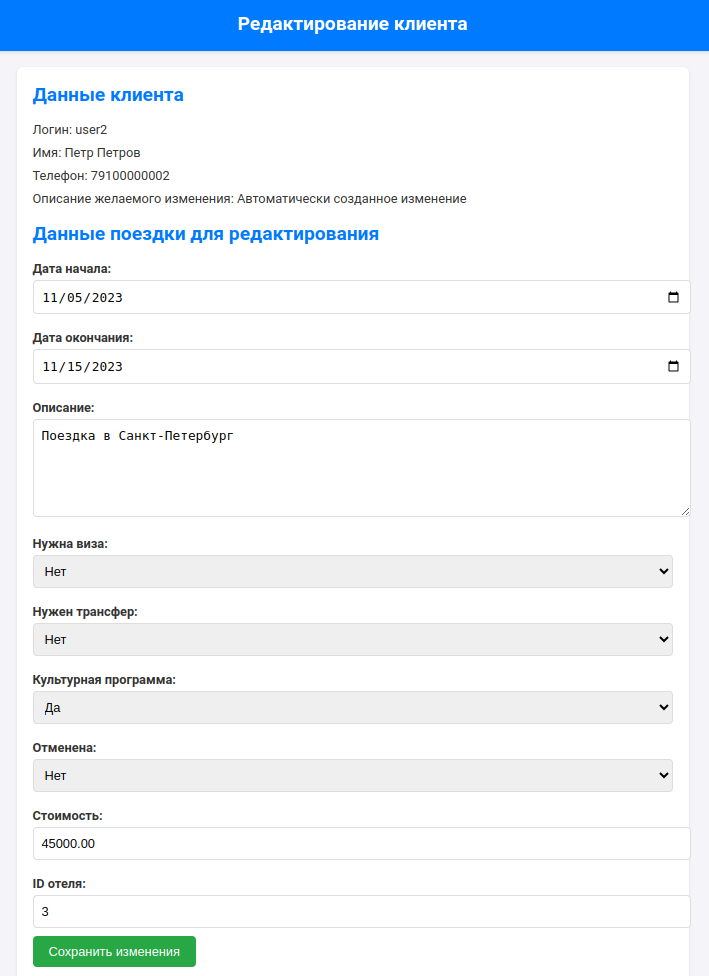
\includegraphics[width=4.552083333333333in, height=6.260415573053368in]{media/edit_trip.png}
\end{itemize}

\subsection{Основной стиль:}

\begin{itemize}
    \item Современный плоский дизайн (Flat Design):
          \begin{itemize}
              \item Прямоугольные формы без сложных градиентов.
              \item Простая, чистая цветовая гамма с акцентами (синий и белый).
              \item Использование теней для элементов (например, box-shadow) для легкой глубины.
              \item Отсутствие излишней декоративности, акцент на функциональности.
              \item Подробнее о Flat Design: \url{https://en.wikipedia.org/wiki/Flat_design}
          \end{itemize}

    \item Материальный дизайн (Material Design):
          \begin{itemize}
              \item Плавные переходы и изменения состояния элементов управления (например, transition: background-color 0.3s ease).
              \item Анимации для наведения (:hover).
              \item Использование карточного стиля для таблиц и других блоков (например, box-shadow и закругленные углы).
              \item Подробнее о Material Design:  \url{https://ru.wikipedia.org/wiki/Material_Design}
          \end{itemize}
\end{itemize}

\subsection{Основные цвета:}

\begin{itemize}
    \item Синий (\#007BFF): акцент для кнопок, ссылок и заголовков.
    \item Белый: фон для элементов.
    \item Серый и черный (\#333, \#ccc): текст и границы.
\end{itemize}

\section{Полный сценарий демонстрации}

\begin{enumerate}
    \item Роль неавторизованный пользователь:
          \begin{itemize}
              \item На странице \texttt{localhost/index.php} пользователь сразу попадает на экран авторизации Рис. 1, а также видит кнопки "войти" и "зарегистрироваться".
          \end{itemize}

    \item Роль клиент:
          \begin{itemize}
              \item (Описание сценария для клиента)
          \end{itemize}

    \item Роль менеджер:
          \begin{itemize}
              \item (Описание сценария для менеджера)
          \end{itemize}
\end{enumerate}


\end{document}